\chapter{Planet Canterbury Christ Church}
\section{Setting up}
Using Mozzila's brilliant AFrame, a web-based Virtual Reality model of a planet with rings and include a moon with an image on it.
The first step is to set a new site in trinket (or use the old one)  and then add a white sphere on a black background.
\begin{lstlisting}
<html>
  <head>
    <script src="https://aframe.io/releases/0.9.2/aframe.min.js"></script>
  </head>
  <body>
    <a-scene>
     <a-sphere position="0 1.25 -5" radius="3" color="white" >
      </a-sphere>   
      <a-sky color="black"></a-sky>
    </a-scene>
  </body>
</html>
\end{lstlisting}

Using the Aframe 'tags' to create a white sphere and to create a black background

\section{Rotate the planet and add some colour}
Now we can add a surface to the planet by finding an appropriate image to wrap around the sphere. in this example, I used the site Solar Systems Scope \url{https://www.solarsystemscope.com/textures/} and downloaded an image of Jupiter's surface \url{https://www.solarsystemscope.com/textures/download/2k_jupiter.jpg}.

 

(a)If you are using Glitch: This needs to be copied into the assets folder of the project and the URL generated (by left-clicking on the image when it is in the folder) copied.

(b)On you own site upload the image to the same folder as the webpage the ‘URL’ will be filename

(c ) Alternatively use this URL in either approach \url{https://cdn.glitch.com/febf6408-3c33-4608-ac90-b087753e5792%2F2k_jupiter.jpg?v=1573393224376}

Now by adding src="" and in the speech-marks paste in the URL for the image; the image wraps around the sphere.
\begin{lstlisting}
<html>
  <head>
    <script src="https://aframe.io/releases/0.9.2/aframe.min.js"></script>
  </head>
  <body>
    <a-scene>
     <a-sphere position="0 1.25 -5" radius="3" color="white" src="https://cdn.glitch.com/febf6408-3c33-4608-ac90-b087753e5792%2F2k_jupiter.jpg?v=1573393224376">
      </a-sphere>   
      <a-sky color="black"></a-sky>
    </a-scene>
  </body>
</html>
\end{lstlisting}

Now to rotate it  add, also within the , section animation="property: rotation; to: 0 360 0; loop: true; dur: 10000" See below:

\begin{lstlisting}
<a-sphere position="0 1.25 -5" radius="3" color="white" src="https://cdn.glitch.com/febf6408-3c33-4608-ac90-b087753e5792%2F2k_jupiter.jpg?v=1573393224376"
               animation="property: rotation; to: 0 360 0; loop: true; dur: 10000">
\end{lstlisting}

\section{planets need rings}
In Aframe if you nest another object with the <></> of another object it's position is set relative to the first object. This principle is going to be used here put a ring around the planet. The first stage is to add the ring object is used for this and a the same rotating animation is used. We are going to use a squashed doughnut shape <a-torus> to do this. When the webpage is running you will probably need use the down arrow key to zoom out to see the ring.

\begin{lstlisting}
<html>
  <head>
    <script src="https://aframe.io/releases/0.9.2/aframe.min.js"></script>
  </head>
  <body>
    <a-scene>
     <a-sphere position="0 1.25 -5" radius="3" color="white" src="https://cdn.glitch.com/febf6408-3c33-4608-ac90-b087753e5792%2F2k_jupiter.jpg?v=1573393224376"
               animation="property: rotation; to: 0 360 0; loop: true; dur: 10000">
        <a-torus position="0 0 0" arc="360"
                rotation="90 0 0"
                color="white" radius="5"
                radius-tubular="0.05"
                animation="property: rotation; to:  90 0 0; loop: true; dur: 3000">
         </a-torus>
      </a-sphere>   
      <a-sky color="black"></a-sky>
    </a-scene>
  </body>
</html>
\end{lstlisting}

DON'T PANIC: It is not expected that you will necessarily understand this all in one go. So experiment now try different values for rotation; to:  90 0 0  for example to:  -360 360 0; and dur: 3000 what changed? 

\begin{figure}
    \centering
    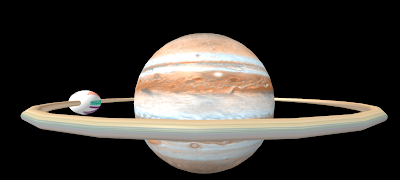
\includegraphics[width=10cm]{chapters/chapter2/figures/Picture1.png}
    \caption{Starting point}
    \label{fig:Picture1}
\end{figure}


\section{It needs a moon}
The process is really just combining elements of the steps 1-3. Create a new sphere,set the radius to something around 0.25 to 0.5; colour it with whatever you feel is appropriate, add an image (in the example code one has been added) if you want, set a rotation (it is is fun to play with these a bit and place the moon on the ring (setting position="5 0 0" in this case does this.

If the images are accessible as web sources this could be a great option.

Lets put a moon on the ring (ie. within the <a-torus> and </a-torus> tags).

So the code for the moon
\begin{lstlisting}
                <a-sphere position="5 0 0"
                 rotation="0 0 0"
                 radius="0.5"
                 color="yellow" src="https://cdn.glitch.com/febf6408-3c33-4608-ac90-b087753e5792%2Fpanic.png?v=1573395380360"
                 animation="property: rotation; to:  0 259 0; loop: true; dur: 3000">
              </a-sphere>
\end{lstlisting}
Gets put inside that of the torus, so the whole thing becomes
\begin{lstlisting}
<html>
  <head>
    <script src="https://aframe.io/releases/0.9.2/aframe.min.js"></script>
  </head>
  <body>
    <a-scene>
     <a-sphere position="0 1.25 -5" radius="3" color="white" src="https://cdn.glitch.com/febf6408-3c33-4608-ac90-b087753e5792%2F2k_jupiter.jpg?v=1573393224376"
               animation="property: rotation; to: 0 360 0; loop: true; dur: 10000">
        <a-torus position="0 0 0" arc="360"
                rotation="90 0 0"
                color="white" radius="5"
                radius-tubular="0.05"
                animation="property: rotation; to:  90 90 0; loop: true; dur: 3000">
                <a-sphere position="5 0 0"
                 rotation="0 0 0"
                 radius="0.5"
                 color="yellow" src="https://cdn.glitch.com/febf6408-3c33-4608-ac90-b087753e5792%2Fpanic.png?v=1573395380360"
                 animation="property: rotation; to:  0 259 0; loop: true; dur: 3000">
              </a-sphere>
         </a-torus>
      </a-sphere>   
      <a-sky color="black"></a-sky>
    </a-scene>
  </body>
</html>               
\end{lstlisting}

\section{Let's add text and stars}
So we might want to put some text into the world we can do that with <a-text value=””> So adding this to the code (see below) put a message on the screen, though you may have to use the down arrow to see it.

\begin{lstlisting}
<html>
  <head>
    <script src="https://aframe.io/releases/0.9.2/aframe.min.js"></script>
  </head>
  <body>
    <a-scene>
     <a-sphere position="0 1.25 -5" radius="3" color="white" src="https://cdn.glitch.com/febf6408-3c33-4608-ac90-b087753e5792%2F2k_jupiter.jpg?v=1573393224376"
               animation="property: rotation; to: 0 360 0; loop: true; dur: 10000">
        <a-torus position="0 0 0" arc="360"
                rotation="90 0 0"
                color="white" radius="5"
                radius-tubular="0.05"
                animation="property: rotation; to:  90 90 0; loop: true; dur: 3000">
                <a-sphere position="5 0 0"
                 rotation="0 0 0"
                 radius="0.5"
                 color="yellow" src="https://cdn.glitch.com/febf6408-3c33-4608-ac90-b087753e5792%2Fpanic.png?v=1573395380360"
                 animation="property: rotation; to:  0 259 0; loop: true; dur: 3000">
              </a-sphere>
         </a-torus>
      </a-sphere>   
      <a-text value="Planet CCCU Computing" position="0 4 -2"></a-text>
      <a-sky color="black"></a-sky>
    </a-scene>
  </body>
</html>
\end{lstlisting}

\begin{figure}
    \centering
    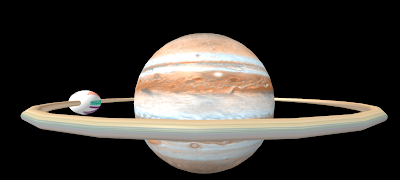
\includegraphics[width=10cm]{chapters/chapter2/figures/Picture1.png}
    \caption{Starting point}
    \label{fig:Planet again}
\end{figure}

We can get interesting effects if we add the text between  </a-sphere> and </a-torus> Try adding this in there. <a-text value="Planet CCCU Computing" position="0 3 -2"></a-text>

Have a play with altering the text and putting the line elsewhere in the code. What happens?

Now going to use an image to change the background. The image is "space" by fleskw is licensed with CC BY 2.0. To view a copy of this license, visit \url{https://creativecommons.org/licenses/by/2.0} You will need to change the sky colour to a light colour for this to work. So change the sky line in the code to white we are going to use the space image to make it a bit easier it is in this form \url{https://cdn.glitch.com/425c1a98-7ba9-463d-817d-6b491a516246%2F97b3bf6d-ced1-4041-80d4-b6c9a98ba43d.jfif?v=1614341330757} 

\begin{lstlisting}
<a-sky color="white" src="https://cdn.glitch.com/425c1a98-7ba9-463d-817d-6b491a516246%2F97b3bf6d-ced1-4041-80d4-b6c9a98ba43d.jfif?v=1614341330757"></a-sky>
\end{lstlisting}
Now adding it the code in place of the current <a-sky> line we 
\begin{lstlisting}
<html>
  <head>
    <script src="https://aframe.io/releases/0.9.2/aframe.min.js"></script>
  </head>
  <body>
    <a-scene>
     <a-sphere position="0 1.25 -5" radius="3" color="white" src="https://cdn.glitch.com/febf6408-3c33-4608-ac90-b087753e5792%2F2k_jupiter.jpg?v=1573393224376"
               animation="property: rotation; to: 0 360 0; loop: true; dur: 10000">
        <a-torus position="0 0 0" arc="360"
                rotation="90 0 0"
                color="white" radius="5"
                radius-tubular="0.05"
                animation="property: rotation; to:  90 90 0; loop: true; dur: 3000">
                <a-sphere position="5 0 0"
                 rotation="0 0 0"
                 radius="0.5"
                 color="yellow" src="https://cdn.glitch.com/febf6408-3c33-4608-ac90-b087753e5792%2Fpanic.png?v=1573395380360"
                 animation="property: rotation; to:  0 259 0; loop: true; dur: 3000">
              </a-sphere>
         </a-torus>
      </a-sphere>   
      <a-text value="Planet CCCU Computing" position="0 4 -2"></a-text>
      <a-sky color="white" src="https://cdn.glitch.com/425c1a98-7ba9-463d-817d-6b491a516246%2F97b3bf6d-ced1-4041-80d4-b6c9a98ba43d.jfif?v=1614341330757"></a-sky>
    </a-scene>
  </body>
</html>
\end{lstlisting}

We are done!

\begin{figure}
    \centering
    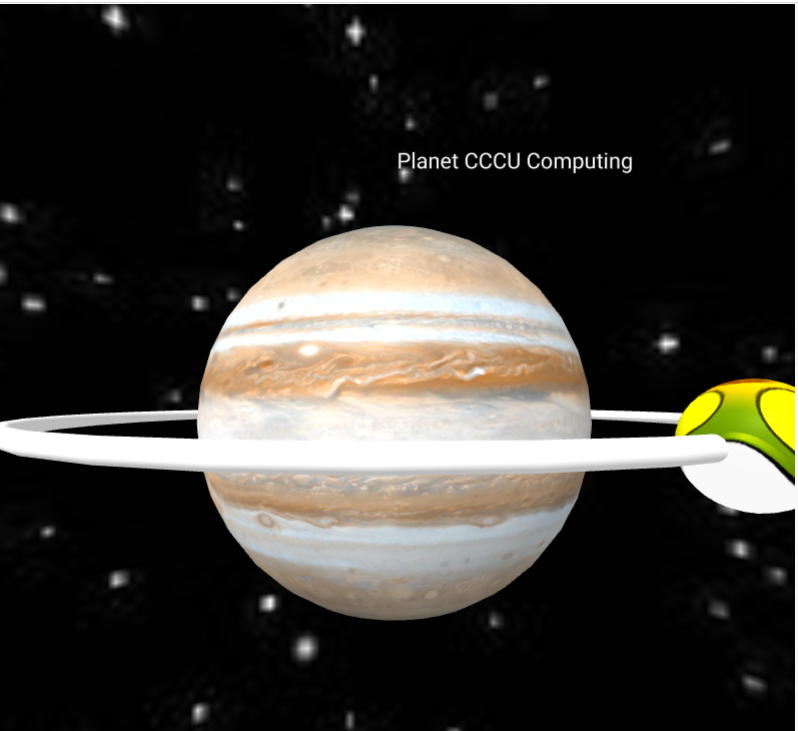
\includegraphics[width=10cm]{chapters/chapter2/figures/planet3.png}
    \caption{Starting point}
    \label{fig:Planet3}
\end{figure}